\documentclass[tikz, border=10pt]{standalone}

\usepackage{tikz}
\usetikzlibrary{shapes.misc} % 'shapes.misc' para formas como 'rounded corners', 'shadow' para la sombra
\usetikzlibrary{calc,angles,quotes}
\usetikzlibrary{decorations.pathmorphing,patterns}
\usetikzlibrary{patterns}
\usetikzlibrary{shapes.geometric, positioning, decorations.pathreplacing, arrows.meta}
\usetikzlibrary{shapes.callouts, positioning, backgrounds, shadows, arrows.meta, fit, shapes.misc, calc}
\usepackage{pgfplots}
\pgfplotsset{compat=1.18} % <--- Esta es la línea mágica
\usepackage{afterpage}
\usetikzlibrary{calc}
\tikzset{dotted lines/.style={black, loosely dotted,  thick}}
\usepackage{amsmath}
\usetikzlibrary{shadings}
\usepackage{circuitikz}
\usetikzlibrary{positioning, calc}
\usetikzlibrary{calc, arrows.meta, decorations.markings}

% --- PREÁMBULO (Colores y Estilos) ---
\usepackage{xcolor}
\usepackage{tikz}
\usetikzlibrary{calc, arrows.meta} % Necesario para tus cálculos de coordenadas

% 1. Definición de la Paleta "Scientific Modern"
\definecolor{ChargePos}{HTML}{E63946} % Rojo vibrante
\definecolor{ChargeNeg}{HTML}{457B9D} % Azul sólido
\definecolor{Charge0}{HTML}{6B7280}
\definecolor{VecForce}{HTML}{1D3557}  % Azul oscuro (Fuerza)
\definecolor{VecDisp}{HTML}{E63946}   % Rojo (Desplazamiento/Posición relativo)
\definecolor{AxisGray}{HTML}{6B7280}  % Gris medio (Ejes/Geometría)
\definecolor{TextGray}{HTML}{374151}  % Gris oscuro (Texto)
\definecolor{SupGauss}{HTML}{F73BC5}

% Colores de relleno suaves (20% de opacidad)
\colorlet{FillPos}{ChargePos!20}
\colorlet{FillNeg}{ChargeNeg!20}
\colorlet{Fill0}{Charge0!20}

% 2. Configuración de Estilos TikZ (Para no repetir código)
\tikzset{
	% Estilo para Carga Positiva (+q)
	charge+/.style={circle, draw=ChargePos, fill=FillPos, very thick, minimum size=8mm, text=black},
	% Estilo para Carga Negativa (-q)
	charge-/.style={circle, draw=ChargeNeg, fill=FillNeg, very thick, minimum size=8mm, text=black},
	% Estilo para Carga Neutra
	charge0/.style={circle, draw=Charge0, fill=Fill0, very thick, minimum size=8mm, text=black},
	% Estilo para Vectores de Fuerza
	force/.style={->, VecForce, ultra thick, >=latex},
	% Estilo para Elementos Geométricos (cotas, líneas punteadas)
	geo/.style={AxisGray, dashed, thick},
	% Estilo para vectores de posición
	posvec/.style={->, AxisGray, thick, >=latex},
	preposvec/.style={<->, AxisGray, thick, >=latex},
	cota/.style={{Straight Barb[]}-{Straight Barb[]}, AxisGray, thick},
	campo/.style={color=red, thick, ->, >=latex,
		axis/.style={->,thick}},
	dot/.style={circle,fill,inner sep=1.5pt}
}

\begin{document}
	\pagestyle{empty}
	
	
%	### Gráficos Cinemáticos del Modelo
%	
%	A continuación, se representan las curvas de velocidad y aceleración en función del tiempo para ambas fases del movimiento. Se puede observar geométricamente cómo el área bajo la curva en el gráfico de velocidad corresponde a los desplazamientos $h_1$ (fase de empuje) y $h_2$ (vuelo libre).
	
%	```{tikz}
	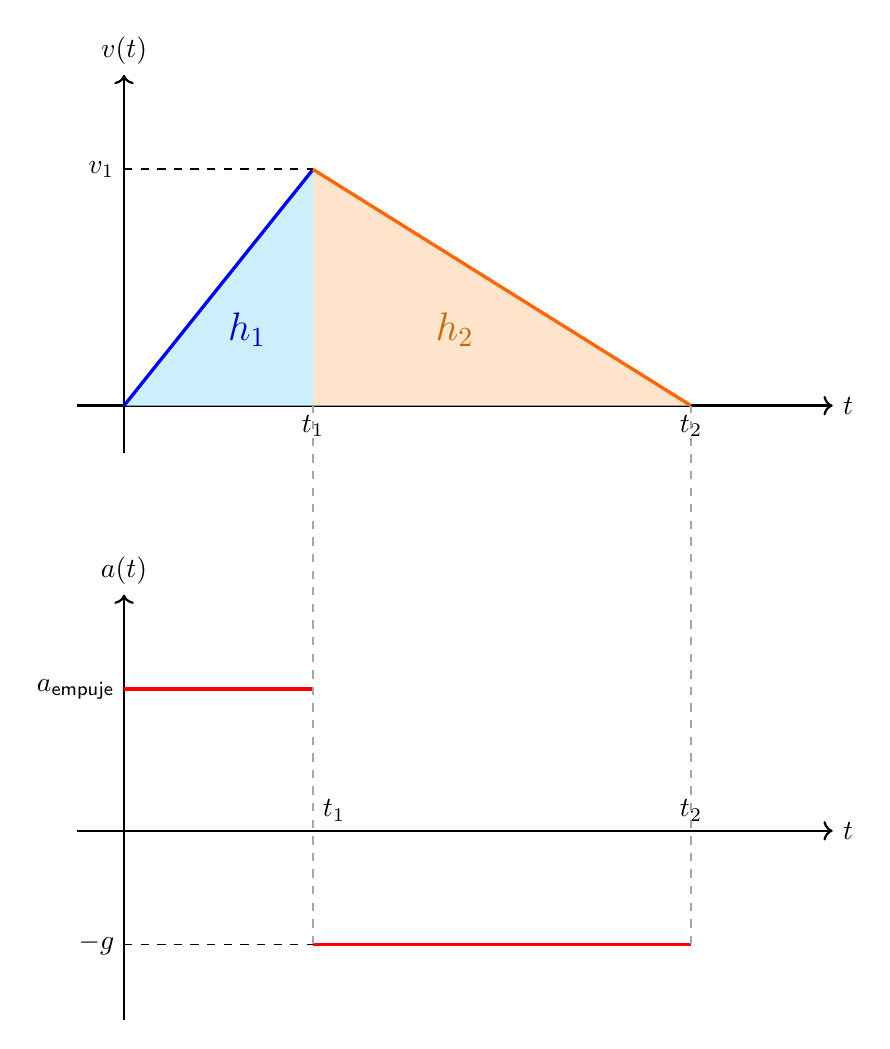
\begin{tikzpicture}[scale=1.2, font=\sffamily]
		
		% ================= GRÁFICO DE VELOCIDAD =================
		\begin{scope}[yshift=4.5cm] % Desplazamiento hacia arriba
			% Ejes
			\draw[->, thick] (-0.5, 0) -- (7.5, 0) node[right] {$t$};
			\draw[->, thick] (0, -0.5) -- (0, 3.5) node[above] {$v(t)$};
			
			% Áreas sombreadas (h1 y h2)
			\fill[cyan!20] (0,0) -- (2,2.5) -- (2,0) -- cycle;
			\fill[orange!20] (2,0) -- (2,2.5) -- (6,0) -- cycle;
			
			% Líneas de la función
			\draw[very thick, blue] (0,0) -- (2,2.5);
			\draw[very thick, orange!80!red] (2,2.5) -- (6,0);
			
			% Líneas punteadas de referencia
			\draw[dashed, thick] (0, 2.5) -- (2, 2.5);
			
			% Textos y Etiquetas
			\node[left] at (0, 2.5) {$v_1$};
			\node[below] at (2, 0) {$t_1$};
			\node[below] at (6, 0) {$t_2$};
			
			% Etiquetas de las áreas
			\node[text=blue!80!black] at (1.3, 0.8) {\Large $h_1$};
			\node[text=orange!80!black] at (3.5, 0.8) {\Large $h_2$};
			
			% Título
%			\node[above] at (3.5, 3.5) {\textbf{Gráfico de Velocidad vs. Tiempo}};
		\end{scope}
		
		% ================= GRÁFICO DE ACELERACIÓN =================
		\begin{scope}[yshift=0cm]
			% Ejes
			\draw[->, thick] (-0.5, 0) -- (7.5, 0) node[right] {$t$};
			\draw[->, thick] (0, -2) -- (0, 2.5) node[above] {$a(t)$};
			
			% Líneas de la función (Aceleración constante a_empuje y luego -g)
			\draw[very thick, red] (0, 1.5) -- (2, 1.5);
			\draw[very thick, red] (2, -1.2) -- (6, -1.2);
			
			% Salto o discontinuidad
%			\draw[dashed, red, thick] (2, 1.5) -- (2, -1.2);
			
			% Líneas punteadas de referencia a los ejes
%			\draw[dashed] (0, 1.5) -- (2, 1.5);
			\draw[dashed] (0, -1.2) -- (2, -1.2);
			
			% Textos y Etiquetas
			\node[left] at (0, 1.5) {$a_{\text{empuje}}$};
			\node[left] at (0, -1.2) {$-g$};
			\node[above right] at (2, 0) {$t_1$};
			\node[above] at (6, 0) {$t_2$};
			
			% Título
%			\node[above] at (3.5, 2.5) {\textbf{Gráfico de Aceleración vs. Tiempo}};
		\end{scope}
		
		% ================= LÍNEAS DE ALINEACIÓN VERTICAL =================
		% Conectan t1 y t_total a través de ambos gráficos para guiar el ojo
		\draw[dashed, gray!70] (2, -1.2) -- (2, 4.5);
		\draw[dashed, gray!70] (6, -1.2) -- (6, 4.5);
		
	\end{tikzpicture}
	
	%	\input{figuras01.tex}
	\newpage
	%	\input{figuras02.tex}
	\newpage
	%	\input{figuras03.tex}
	\newpage
	%	\input{figuras04.tex}
	\newpage
	%	\input{figuras05.tex}
	\newpage
	%	\input{figuras06.tex}
	\newpage
	%	\input{figuras07.tex}
	\newpage
%	\input{figuras08.tex}
	\newpage
	%	\input{figuras09.tex}
	\newpage
	%	\input{figuras10.tex}
	\newpage
	%	\input{figuras11.tex}
	\newpage
	%	\input{figuras12.tex}
\end{document}

